\documentclass[12pt]{article}
\usepackage{tikz}
\usetikzlibrary{arrows.meta}
\usetikzlibrary{arrows.meta, positioning}
\usetikzlibrary{shapes, positioning}
\usetikzlibrary{calc}
\usepackage[T1]{fontenc}
\usepackage[margin=2cm]{geometry}

\usepackage{amssymb}
\usepackage{amsmath}
\usepackage{tcolorbox}
\usepackage{xcolor}
\usepackage{framed}
\usepackage{euscript}
\usepackage{float}

\usepackage{verbatim}
\usepackage{mathrsfs}
\usepackage{graphicx}
\usepackage{multicol}

\usepackage{bbm,txfonts}
\usepackage{float}


\usepackage{titletoc}
\usepackage{tikz}
\usepackage{xspace}

\usepackage{enumitem}

\newcommand{\answer}{\vspace*{4pt} \noindent{\bf Solution: }}

\newcommand{\bb}[1]{\mathbb{#1}}
\renewcommand{\v}[1]{\boldsymbol{#1}}
\newcommand{\m}[1]{\mathbf{#1}}
\renewcommand{\c}[1]{\mathcal{#1}}
\usepackage{upquote}


\renewcommand{\tilde}{\widetilde}
\newcommand{\halmos}{\vspace{3mm} \hfill \mbox{$\Box$}}

\newcommand{\Var}{\mathbb{V}\mathrm{ar}}
\newcommand{\var}{\Var}

\newcommand{\Cov}{\mathbb{C}\mathrm{ov}}
\newcommand{\cov}{\Cov}

\renewcommand{\epsilon}{\varepsilon}
\renewcommand{\rho}{\varrho}
\renewcommand{\log}{\ln}
\renewcommand{\hat}{\widehat}

\newcommand{\iid}{\text{iid }}


% Bernoulli distribution
\newcommand{\Ber}{{\sf Ber}}
\newcommand{\ber}{\Ber}

% Binomial distribution
\newcommand{\Bin}{{\sf Bin}}
\newcommand{\bin}{\Bin}

% Cauchy distribution
\newcommand{\Cauchy}{{\sf Cauchy}}

% Negative binomial distribution
\newcommand{\NegBin}{{\sf NegBin}}

% Multinomial distribution
\newcommand{\Mnom}{{\sf Mnom}}
\newcommand{\mnom}{\Mnom}

% Geometric distribution
\newcommand{\Geo}{{\sf Geom}}
\newcommand{\geo}{\Geo}
\newcommand{\Geom}{\Geo}
\newcommand{\geom}{\Geo}
\newcommand{\G}{\Geo}

% Hypergeometric distribution
\newcommand{\Hyp}{{\sf Hyp}}

% Poisson distribution
\newcommand{\Poi}{{\sf Poi}}
\newcommand{\poi}{\Poi}
\newcommand{\Po}{\Poi}
\newcommand{\po}{\Poi}

% Uniform distribution (continuous)
\newcommand{\U}{\EuScript{U}}

% Exponential distribution
\newcommand{\Ex}{{\sf Exp}}
\newcommand{\ex}{\Ex}

% Normal / Gaussian distribution
\newcommand{\Nor}{\EuScript{N}}
\newcommand{\nor}{\Nor}

% Pareto distribution
\newcommand{\Pareto}{{\sf Pareto}}
\newcommand{\pareto}{\Pareto}

% Negative hypergeometric distribution
\newcommand{\NegHyp}{{\sf NegHyp}}

% Student's t distribution
\newcommand{\Student}{{\sf t}}
\newcommand{\student}{\Student}

% Gamma distribution
\newcommand{\Gam}{{\sf Gamma}}
\newcommand{\gam}{\Gam}

% Discrete uniform distribution
\newcommand{\DU}{{\sf DU}}

% Generic distribution
\newcommand{\Dist}{{\sf Dist}}

\newcommand{\Em}{{\mathbb E}}  % expectation
\newcommand{\Pm}{{\mathbb P}}  % probability measure
\newcommand{\R}{{\mathbb R}}

\newcommand{\gvn}{\,|\,}  % conditional (given)

\newcommand{\e}{\mathrm{e}} %Euler's e

\newcommand{\ds}{\displaystyle}

\newcommand{\di}{\mathrm{d}}  % use for differential symbol


\newcommand{\approxsim}{\stackrel{\mathrm{approx.}}{\sim}}

\newcommand{\iidsim}{\stackrel{\mathrm{iid}}{\sim}}
\newcommand{\simiid}{\iidsim}
\newcommand{\simiidt}{{\:{\sim}_{\mathrm{iid}}\:}}

%% Correlation
\newcommand{\Corr}{\mathrm{Corr}}
\newcommand{\corr}{\Corr}


\usepackage{cprotect}
\RequirePackage[formats]{listings}\RequirePackage{textcomp}

\lstnewenvironment{Pout}{%
  \lstset{backgroundcolor=\color{outcol},
  aboveskip= -2pt,  
  xleftmargin = 4pt,
  xrightmargin = 4pt,
  frame=single,
  upquote,
  framerule=1pt,
  basicstyle=\footnotesize\ttfamily,
  columns=fixed}}{}

%DK: See http://latexcolor.com/
\definecolor{applegreen}{rgb}{0.55, 0.41, 0.0}
\definecolor{gray1}{rgb}{0.98, 0.98, 0.98}
\definecolor{black}{rgb}{0, 0, 0}
\definecolor{cream}{rgb}{1.0, 0.99, 0.82}
\definecolor{islamicgreen}{rgb}{0.0, 0.56, 0.0}
\definecolor{vlgray}{gray}{0.9}
\definecolor{lgray}{gray}{0.7}
\definecolor{outcol}{gray}{0.9}

\tcbuselibrary{listings,skins,breakable,theorems}

\newenvironment{PC}{%
\tcblisting{breakable,listing only,colback=cream, enhanced, sharpish
corners,  boxrule=1pt,after, listing options =
   {language=Python,
  basicstyle=\footnotesize\ttfamily,        % the size of the fonts that are used for the code
  numbers=none,                   % where to put the line-numbers
%  numberstyle=\tiny\color{blue},  % the style that is used for the line-numbers
  xleftmargin=-10pt,
  aboveskip=-4pt,
  belowskip=-6pt,
  columns=fixed,
  basewidth=5pt,                     %separation of letters
%  stepnumber=1,                % the step between two line-numbers. If it's 1, each line will be numbered
%  numbersep=7pt,                  % how far the line-numbers are from the code
  backgroundcolor=\color{cream},  % choose the background color. You must add \usepackage{color}
  showspaces=false,               % show spaces adding particular underscores
  showstringspaces=false,         % underline spaces within strings
  showtabs=false,                 % show tabs within strings adding particular underscores
  %frame=single,                   % adds a frame around the code
  %frame=shadowbox,
  %rulecolor=\color{black},        % if not set, the frame-color may be changed on line-breaks within not-black text (e.g. comments (green here))
  tabsize=2,                     % sets default tabsize to 2 spaces
 % captionpos=b,                  % sets the caption-position to bottom
  breaklines=true,                % sets automatic line breaking
  breakatwhitespace=false,        % sets if automatic breaks should only happen at whitespace
  %title=\lstname,                 % show the filename of files included with \lstinputlisting;
                                  % also try caption instead of title
  keywordstyle=\color{blue},      % keyword style
  upquote,     % very important to get right quote for cut/paste
  commentstyle=\color{islamicgreen},   % comment style
  stringstyle=\color{red},      % string literal style
 % escapeinside={\%*}{*)},         % if you want to add a comment within your code
  morekeywords={*,...}
  			 }
    		}
    	}
{\endtcblisting}







\begin{document}
\begin{center}

{\Large  {\bf Mathematical Probability (STAT2003/STAT7003)}

Assignment 3 - Semester 1, 2025.

}
\end{center}

The due date/time is given on Blackboard. STAT7003 students have additional items,\\ marked with a ``{\bf (*STAT7003)}''. The assignment has 5 questions with multiple items per question. Note that STAT7003 students (master's) need to complete all items. In contrast, {\bf STAT2003 students will only be marked on items not marked as STAT7003}. The weighting of the items is indicated in each question.\\ 


\begin{enumerate}

%%%%%%%%%%%%%%%%%%%%
% Q1
%%%%%%%%%%%%%%%%%%%%
\item Let $X_1 \sim \Nor(\mu_1, \sigma^2)$ and $X_2 \sim \Nor(\mu_2, \sigma^2)$ be independent random variables. Consider $Y_1 = X_1+X_2$ and $Y_2 = X_1-X_2$.   

\begin{enumerate}
\item Using moment generating function (MGF), show that $Y_1$ and $Y_2$ are independent. \\
\emph{Note:} You may use the fact that the joint MGF of independent random variables is the product of the individual MGFs. 
			\hfill [7 marks]
%
\\
\textbf{Answer:}
\\
The moment generating function (MGF) of a normal random variable $X \sim \Nor(\mu, \sigma^2)$ is given by:
\[
M_X(t) = \exp\left(\mu t + \frac{\sigma^2 t^2}{2}\right)
\]
Thus, the MGFs of $X_1$ and $X_2$ are:
\[
M_{X_1}(t) = \exp\left(\mu_1 t + \frac{\sigma^2 t^2}{2}\right)
\]
\[
M_{X_2}(t) = \exp\left(\mu_2 t + \frac{\sigma^2 t^2}{2}\right)
\]
The joint MGF of $X_1$ and $X_2$ is given by:
\[
M_{X_1, X_2}(t_1, t_2) = M_{X_1}(t_1) \cdot M_{X_2}(t_2) = \exp\left(\mu_1 t_1 + \frac{\sigma^2 t_1^2}{2}\right) \cdot \exp\left(\mu_2 t_2 + \frac{\sigma^2 t_2^2}{2}\right)
\]
Now, we can express $Y_1$ and $Y_2$ in terms of $X_1$ and $X_2$:
\[
Y_1 = X_1 + X_2
\]
\[
Y_2 = X_1 - X_2
\]
To find the joint MGF of $Y_1$ and $Y_2$, we need to express $X_1$ and $X_2$ in terms of $Y_1$ and $Y_2$. We can do this by solving the equations:
\[
X_1 = \frac{Y_1 + Y_2}{2}
\]
\[
X_2 = \frac{Y_1 - Y_2}{2}
\]
Substituting these expressions into the joint MGF of $X_1$ and $X_2$, we get:
\[
M_{Y_1, Y_2}(t_1, t_2) = M_{X_1, X_2}\left(\frac{t_1 + t_2}{2}, \frac{t_1 - t_2}{2}\right)
\]
Substituting the MGFs of $X_1$ and $X_2$, we have:
\[
M_{Y_1, Y_2}(t_1, t_2) = \exp\left(\mu_1 \frac{t_1 + t_2}{2} + \frac{\sigma^2}{2}\left(\frac{t_1 + t_2}{2}\right)^2\right) \cdot \exp\left(\mu_2 \frac{t_1 - t_2}{2} + \frac{\sigma^2}{2}\left(\frac{t_1 - t_2}{2}\right)^2\right)
\]
Now, we can simplify this expression:
\[
M_{Y_1, Y_2}(t_1, t_2) = \exp\left(\frac{\mu_1 + \mu_2}{2} t_1 + \frac{\mu_1 - \mu_2}{2} t_2 + \frac{\sigma^2}{8}\left(t_1^2 + t_2^2 + 2t_1 t_2\right) + \frac{\sigma^2}{8}\left(t_1^2 - t_2^2 - 2t_1 t_2\right)\right)
\]
This simplifies to:
\[
\boxed {M_{Y_1, Y_2}(t_1, t_2) = \exp\left(\frac{\mu_1 + \mu_2}{2} t_1 + \frac{\mu_1 - \mu_2}{2} t_2 + \frac{\sigma^2}{4} t_1^2 + \frac{\sigma^2}{4} t_2^2\right)}
\]
This is the joint MGF of $Y_1$ and $Y_2$. This can also be expressed as the product of the individual MGFs:
\[
M_{Y_1, Y_2}(t_1, t_2) = \exp\left(\frac{\mu_1 + \mu_2}{2} t_1 + \frac{\sigma^2}{4} t_1^2 \right) \cdot \exp\left(\frac{\mu_1 - \mu_2}{2} t_2 + \frac{\sigma^2}{4} t_2^2\right)
\]
\[
= M_{Y_1}(t_1) \cdot M_{Y_2}(t_2)
\]

Since the joint MGF can be expressed as a product of the individual MGFs, we conclude that $Y_1$ and $Y_2$ are independent random variables.


\item Find the joint probability density function (PDF) of $Y_1$ and $Y_2$. 
			\hfill [3 marks]
%
\\
\textbf{Answer:}
\\

The joint PDF of $X_1$ and $X_2$ is given by the product of their individual PDFs:
\begin{align*}
f_{X_1, X_2}(x_1, x_2) &= f_{X_1}(x_1) \cdot f_{X_2}(x_2) \\
&= \frac{1}{\sqrt{2\pi \sigma^2}} \exp\left(-\frac{(x_1 - \mu_1)^2}{2\sigma^2}\right) \cdot \frac{1}{\sqrt{2\pi \sigma^2}} \exp\left(-\frac{(x_2 - \mu_2)^2}{2\sigma^2}\right) \\
&= \frac{1}{2\pi \sigma^2} \exp\left(-\frac{(x_1 - \mu_1)^2 + (x_2 - \mu_2)^2}{2\sigma^2}\right)
\end{align*}

The transformation from $(X_1, X_2)$ to $(Y_1, Y_2)$ is given by the equation:
\begin{align*}
f_{Y_1, Y_2}(y_1, y_2) &= f_{X_1, X_2}\left(x_1,x_2\right) \cdot \left|J\right| \\
\end{align*}

The Jacobian of the transformation is given by:
\begin{align*}
J &= \begin{vmatrix}
\frac{\partial x_1}{\partial y_1} & \frac{\partial x_1}{\partial y_2} \\
\frac{\partial x_2}{\partial y_1} & \frac{\partial x_2}{\partial y_2}
\end{vmatrix} \\
&= \begin{vmatrix}
\frac{1}{2} & \frac{1}{2} \\
\frac{1}{2} & -\frac{1}{2}
\end{vmatrix} \\
&= \left(\frac{1}{2}\right)\left(-\frac{1}{2}\right) - \left(\frac{1}{2}\right)\left(\frac{1}{2}\right) \\
&= -\frac{1}{4} - \frac{1}{4} \\
&= -\frac{1}{2}
\end{align*}

Thus, the absolute value of the Jacobian is $|J| = \frac{1}{2}$.
Now, we can express the joint PDF of $Y_1$ and $Y_2$ as:

\begin{align*}
f_{Y_1, Y_2}(y_1, y_2) &= f_{X_1, X_2}\left(\frac{y_1 + y_2}{2}, \frac{y_1 - y_2}{2}\right) \cdot \left|J\right| \\
&= \frac{1}{2\pi \sigma^2} \exp\left(-\frac{\left(\frac{y_1 + y_2}{2} - \mu_1\right)^2 + \left(\frac{y_1 - y_2}{2} - \mu_2\right)^2}{2\sigma^2}\right) \cdot \frac{1}{2} \\
\end{align*}

This simplifies to:
\[
\boxed{f_{Y_1, Y_2}(y_1, y_2) = \frac{1}{4\pi \sigma^2} \exp\left(-\frac{\left(\frac{y_1 + y_2}{2} - \mu_1\right)^2 + \left(\frac{y_1 - y_2}{2} - \mu_2\right)^2}{2\sigma^2}\right)}
\]

This is the joint PDF of $Y_1$ and $Y_2$, which is a bivariate normal distribution with means $\mu_1$ and $\mu_2$, and variance $\sigma^2$.
%

\end{enumerate}

%%%%%%%%%%%%%%%%%%%%
\vspace{5pt}
% Q2
%%%%%%%%%%%%%%%%%%%%
\item 
Two machines, A and B, participate in a performance test where each is timed to complete a specific task. The time it takes a machine to complete the task follows a geometric distribution with success probability $p$ per minute; that is, in each minute, there is a probability $p$ that the machine completes the task. Please use the parameterisation of the geometric distribution given in the course notes.  

Let $A$ and $B$ denote the number of minutes taken by machines A and B, respectively, to complete the task. Consider
\begin{itemize}
\item $X=\min(A, B)$: the earliest time the task is completed by either machine,
\item $Y = A-B$: the difference in completion times, and 
\item $Z = \frac{A}{A+B}$: the proportion of total time taken by machine A.
\end{itemize}
 
\begin{enumerate}
\item Find the joint probability mass function (PMF) of $X$ and $Y$. 
			\hfill [8 marks]
%
\\
\textbf{Answer:}
\\
The probability disibutions of $A$ and $B$ are given by:
\begin{align*}
P(A=a) &= (1-p)^{a-1}p \quad \text{for } k=1,2,\ldots \\
P(B=b) &= (1-p)^{b-1}p \quad \text{for } k=1,2,\ldots
\end{align*}

We break the problem into two cases - when $a\geq b$ and when $a<b$.

\subsubsection*{Case 1: $a\geq b$, $y \geq 0$}

In this case, we have $X = b$ and $Y = a-b$. The joint PMF is given by:
\begin{align*}
P(X=x, Y=y) &= P(A = x + y, B=x) \\
&= P(A = x+y) \cdot P(B=x) \\
&= (1-p)^{(x+y)-1}p \cdot (1-p)^{x-1}p \\
&= \boxed{p^2(1-p)^{2x+y-2}} \\
\end{align*}

\subsubsection*{Case 2: $a<b$, $y < 0$}
In this case, we have $X = a$ and $Y = a-b$. The joint PMF is given by:
\begin{align*}
P(X=x, Y=y) &= P(A = x, B=x-y) \\
&= P(A = x) \cdot P(B=x-y) \\
&= (1-p)^{x-1}p \cdot (1-p)^{(x-y)-1}p \\
&= \boxed{p^2(1-p)^{2x-y-2}} \\
\end{align*}

Therefore, the joint PMF of $X$ and $Y$ is given by:
\begin{align*}
P(X=x, Y=y) &= \begin{cases}
p^2(1-p)^{2x+y-2} & \text{if } y \geq 0 \\
p^2(1-p)^{2x-y-2} & \text{if } y < 0
\end{cases}
\end{align*}


\item Are $X$ and $Y$ independent? Justify your answer.  
			\hfill [2 marks]
%
\\
\textbf{Answer:}
\\
To check if $X$ and $Y$ are independent, we need to see if the joint PMF can be expressed as the product of the marginal PMFs.
The marginal PMF of $X$ can be found by summing the joint PMF over all possible values of $Y$:

\begin{align*}
P(X=x) &= \sum_{y=-\infty}^{\infty} P(X=x, Y=y) \\
&= \sum_{y=0}^{\infty} p^2(1-p)^{2x+y-2} + \sum_{y=-\infty}^{-1} p^2(1-p)^{2x-y-2} \\
&= p^2(1-p)^{2x-2} \sum_{y=0}^{\infty} (1-p)^{y} + p^2(1-p)^{2x-2} \sum_{y=-\infty}^{-1} (1-p)^{-y} \\
\end{align*}

The left sum is a geometric series with the first term $1$ and common ratio $(1-p)$, which converges:

\begin{align*}
\sum_{y=0}^{\infty} (1-p)^{y} &= \frac{1}{p} \\
\end{align*}

The right sum can be rexpressed as:

\begin{align*}
\sum_{y=-\infty}^{-1} (1-p)^{-y} &= \sum_{k=1}^{\infty} (1-p)^{k} \\
&= \frac{(1-p)}{p} \\
\end{align*}

Subsituting these results back into the marginal PMF of $X$, we have:
\begin{align*}
P(X=x) &= p^2(1-p)^{2x-2} \left(\frac{1}{p} + \frac{1-p}{p}\right) \\
&= p(1-p)^{2x-2} \left( 2-p \right) \\
\end{align*}

The marginal PMF of $Y$ can be found similarly by summing the join PMF over all possible values of $X$:

\begin{align*}
P(Y=y) &= \sum_{x=-\infty}^{\infty} P(X=x, Y=y) \\
&= \begin{cases}
\sum_{x=1}^{\infty} p^2(1-p)^{2x+y-2} & \text{if } y \geq 0 \\
\sum_{x=1}^{\infty} p^2(1-p)^{2x-y-2} & \text{if } y < 0
\end{cases}	\\
&= \begin{cases}
	p^2(1-p)^{y} \sum_{x=1}^{\infty} (1-p)^{2x-2} & \text{if } y \geq 0 \\
	p^2(1-p)^{-y} \sum_{x=1}^{\infty} (1-p)^{2x-2} & \text{if } y < 0
\end{cases} \\
\end{align*}

For the sum term, let $k=x-1$ The sum term is a geometric series with the first term $1$ and common ratio $(1-p)^2$, which converges:

\begin{align*}
\sum_{k=0}^{\infty} (1-p)^{2k} &= \frac{1}{p(2-p)} \\
\end{align*}

Substituting this result back into the marginal PMF of $Y$, we have:
\begin{align*}
P(Y=y) &= \begin{cases}
p(1-p)^{y} \left(\frac{1}{p(2-p)}\right) & \text{if } y \geq 0 \\
p(1-p)^{-y} \left(\frac{1}{p(2-p)}\right) & \text{if } y < 0
\end{cases} \\
&= \begin{cases}
\frac{p(1-p)^{y}}{2-p} & \text{if } y \geq 0 \\
\frac{p(1-p)^{-y}}{2-p} & \text{if } y < 0
\end{cases}
\end{align*}

Now, we can check if the joint PMF can be expressed as the product of the marginal PMFs:

\begin{align*}
P(X=x, Y=y) &= \begin{cases}
\frac{p(1-p)^{y}}{2-p} p(1-p)^{2x-2} \left( 2-p \right) & \text{if } y \geq 0 \\
\frac{p(1-p)^{-y}}{2-p} p(1-p)^{2x-2} \left( 2-p \right) & \text{if } y < 0
\end{cases} \\
&= \begin{cases}
p^2(1-p)^{2x+y-2} & \text{if } y \geq 0 \\
p^2(1-p)^{2x-y-2} & \text{if } y < 0
\end{cases} \\
\end{align*}

We can see that the joint PMF can be expressed as the product of the marginal PMFs, which means that $X$ and $Y$ are independent random variables. Therefore, we conclude that $X$ and $Y$ are independent.
%

\item Determine the joint PMF of $A$ and $A+B$. 
			\hfill [4 marks]
%
\\
\textbf{Answer:}
\\
Let $M = A + B$. The joint PMF of $A$ and $M$ can be found by the following:

\begin{align*}
P(A=a, M=m) &= P(A=a, A+B=m) \\
&= P(A=a, B=m-a) \\
&= P(A=a) \cdot P(B=m-a) \\
&= (1-p)^{a-1}p \cdot (1-p)^{(m-a)-1}p \\
&= \begin{cases}
p^2(1-p)^{m-2} \quad \text{for } a=1,2,\ldots,\ m=2,3,\ldots,\ 1 < a < m \\
0 \quad \text{otherwise}
\end{cases} \\
\end{align*}
%

\item Find the PMF of $Z$.  
			\hfill [6 marks]
%
\\
\textbf{Answer:}
\\
Let $Z = \frac{A}{M}$, where $M = A + B$. The PMF of $Z$ can be found by the following:

\begin{align*}
  P(Z=z) &= P\left(\frac{A}{M} = z\right) \\
  &= P\left(A = zM\right) \\
  &= \sum_{m=2}^{\infty} \Pm(Z=z | M=m) \cdot \Pm(M=m) \\
\end{align*}

The conditional PMF $\Pm(Z=z | M=m)$ can be expressed as:
\begin{align*}
  \Pm(Z=z | M=m) &= \Pm(A = a | A + B = m) \\
  &= \frac{\Pm(A = a, A + B = m)}{\Pm(A + B = m)} \\
  &= \frac{p^2(1-p)^{m-2}}{p^2(1-p)^{m-2}} \\
  &= 1
\end{align*}

The marginal PMF $\Pm(M=m)$ can be expressed as:
\begin{align*}
  \Pm(M=m) &= \sum_{a=1}^{m-1} P(A=a, A + B = m) \\
  &= \sum_{a=1}^{m-1} p^2(1-p)^{m-2} \\
  &= (m-1)p^2(1-p)^{m-2}
\end{align*}

Substituting these results back into the PMF of $Z$, we have:
\begin{align*}
  P(Z=z) &= \sum_{m=2}^{\infty} 1 \cdot (m-1)p^2(1-p)^{m-2} \\
  &= p^2 \sum_{m=2}^{\infty} (m-1)(1-p)^{m-2} \\
\end{align*}

If we let $k = m-2$, then we can rewrite the sum as:

\begin{align*}
  P(Z=z) &= p^2 \sum_{k=0}^{\infty} (k+1)(1-p)^{k} \\
  &= p^2 \left(\frac{1}{(1-(1-p))^2}\right) \\
  &= p^2 \left(\frac{1}{p^2}\right) \\
  &= 1
\end{align*}

Thus, the PMF of $Z$ is given by:

The possible values of $Z$ are in the range $[0, 1]$, and the PMF is uniform over this range. Therefore, we can express the PMF of $Z$ as:

\begin{align*}
  P(Z=z) &= \begin{cases}
    1 & \text{if } 0 \leq z \leq 1 \\
    0 & \text{otherwise}
\end{cases}
\end{align*}

%


\item{\bf (*STAT7003)} 
Suppose the test is repeated independently $N$ times. Let $N_A$ be the number of times machine A completes the task before machine B. What is the distribution of $N_A$? What is the probability that machine A is faster than machine B in more than half of the $N$ trials?
			\\\phantom{1}\hfill [10 marks]
%
\\
\textbf{Answer:}
\\
The number of times machine A completes the task before machine B in $N$ trials is given by the expression:

\begin{align*}
N_A &= \sum_{i=1}^{N} I_i \\
I_i &= \begin{cases}
1 & \text{if machine A is faster than machine B in trial } i \\
0 & \text{otherwise}
\end{cases}
\end{align*}

Therefore, $N_A$ is the sum of $N$ independent Bernoulli random variables, where each $I_i$ has a success probability of $p$.
The distribution of $N_A$ is given by the binomial distribution with parameters $N$ and $p$:

\begin{align*}
N_A \sim \mathrm{Binomial}(N, p) \\
\end{align*}


\end{enumerate}

%%%%%%%%%%%%%%%%%%%%
\vspace{5pt}
% Q3
%%%%%%%%%%%%%%%%%%%%
\item An engineer needs to simplify the processing of sensor data by rounding the recorded values to the nearest whole number. For example, both sensor readings of 9.53 and 10.47 will be rounded to 10. To model the rounding errors, the engineer assumes that the rounding errors are independent and follow a uniform distribution between -0.5 and 0.5. Let $X_1, X_2, \ldots, X_n$ represent the rounding errors for $n$ measurements.  

\begin{enumerate}
\item Find the expected value and variance of each rounding error $X_i$.
			\hfill [2 marks]
%
\\
\textbf{Answer:}
\\
The expected value of a uniform distribution $X \sim U(a, b)$ is given by:
\begin{align*}
E[X] &= \frac{a + b}{2} \\
&= \frac{-0.5 + 0.5}{2} \\
&= 0 \\
\end{align*}

The variance of a uniform distribution $X \sim U(a, b)$ is given by:
\begin{align*}
Var[X] &= \frac{(b - a)^2}{12} \\
&= \frac{(0.5 - (-0.5))^2}{12} \\
&= \frac{(1)^2}{12} \\
&= \frac{1}{12} \\
\end{align*}
%

\item Using Chebyshev's inequality, calculate an upper bound for the probability that the total rounding error exceeds 10\% of the number of measurements, that is, $\Pm\left(|\sum_{i=1}^n X_i| > 0.1 n\right)$. 
			\\\phantom{1}\hfill [2 marks]
%
\\
\textbf{Answer:}
\\
The Chebyshev's inequality is given by:
\begin{align*}
\Pm\left(|X - \mu| \geq k\sigma\right) &\leq \frac{1}{k^2}
\end{align*}

where $X$ is a random variable, $\mu$ is the mean of $X$, $\sigma$ is the standard deviation of $X$, and $k$ is a positive constant.

We can apply Chebyshev's inequality to the sum of the rounding errors:

\begin{align*}
\Pm\left(\left|\sum_{i=1}^n X_i - E\left[\sum_{i=1}^n X_i\right]\right| > 0.1 n\right) \\
\end{align*}

Since each $X_i$ has an expected value of $0$, and using the linearity of expectation, we have:

\begin{align*}
\Pm\left(\left|\sum_{i=1}^n X_i - E\left[\sum_{i=1}^n X_i\right]\right| > 0.1 n\right) &= \Pm\left(\left|\sum_{i=1}^n X_i\right| > 0.1 n\right) \\
\end{align*}

If $k\sigma = 0.1 n$, then we can express $k$ as:
\begin{align*}
k &= \frac{0.1 n}{\sigma} \\
&= \frac{0.1 n}{\sqrt{\frac{1}{12}}} \\
&= 0.1 n \sqrt{12} \\
\end{align*}

Therefore, we can apply Chebyshev's inequality:
\begin{align*}
\Pm\left(\left|\sum_{i=1}^n X_i\right| > 0.1 n\right) &\leq \frac{1}{k^2} \\
&= \frac{1}{(0.1 n \sqrt{12})^2} \\
&= \frac{25}{3 n^2} \\
\implies \Pm\left(\left|\sum_{i=1}^n X_i\right| > 0.1 n\right) &\leq \frac{25}{3 n^2} \\
\end{align*}
%

\item A researcher is interested in how the mean absolute error (MAE) $\frac{1}{n} \sum_{i=1}^n |X_i|$ behaves as the number of measurements $n$ becomes large. What can you conclude using the law of large numbers?
			\hfill [4 marks]
%
\\
\textbf{Answer:}
\\
The law of large numbers states that as the number of measurements $n$ increases, the sample mean converges to the expected value of the random variable. In this case, we have:
\begin{align*}
\frac{1}{n} \sum_{i=1}^n |X_i| &\xrightarrow{P} E[|X_i|] \\
\end{align*}

The expected value of the absolute value of a uniform distribution $X \sim U(a, b)$ is given by:
\begin{align*}
E[|X|] &= \frac{1}{b-a} \int_a^b |x| dx \\
&= \frac{1}{b-a} \left(\frac{b^2}{2} - \frac{a^2}{2}\right) \\
&= \frac{1}{b-a} \left(\frac{(0.5)^2}{2} - \frac{(-0.5)^2}{2}\right) \\
&= \frac{1}{b-a} \left(\frac{0.25}{2} - \frac{0.25}{2}\right) \\
&= \frac{1}{b-a} \left(0\right) \\
&= 0 \\
\end{align*}

Therefore, as $n$ becomes large, the mean absolute error converges to the expected value of the absolute value of the rounding error $X_i$, which is $0$. This means that the mean absolute error approaches $0$ as the number of measurements increases.
%

\item For large $n$, find the distribution of the MAE using the central limit theorem. 
			\hfill [2 marks]
%
\\
\textbf{Answer:}
\\
The mean absolute error (MAE) is given by:
\begin{align*}
MAE &= \frac{1}{n} \sum_{i=1}^n |X_i|
\end{align*}

The central limit theorem is says that for large number of independent measurements, the distribution of the sample mean (or also the MAE) approaches a normal distribution. Specifically, it states that:

\begin{align*}
\frac{\bar{X} - \mu}{\sigma/\sqrt{n}} &\xrightarrow{D} N(0, 1)
\end{align*}

Where $\bar{X} = \frac{1}{n} \sum_{i=1}^n |X_i|$ is population mean, $\mu = \Em[|X_i|]$ is the sample mean, and $\sigma = \sqrt{\var[X_i]}$ is the standard deviation of the sample.

We already know that $\mu = 0$ and $\sigma = \sqrt{\frac{1}{12}}$. Therefore, we can the distribution of the MAE as:

\begin{align*}
\frac{MAE - 0}{\sqrt{\frac{1}{12}}/\sqrt{n}} &\xrightarrow{D} N(0, 1) \\
\frac{MAE}{\sqrt{\frac{1}{12}}/\sqrt{n}} &\xrightarrow{D} N(0, 1) \\
MAE &\xrightarrow{D} N\left(0, \frac{1}{12n}\right) \\
\end{align*}
%

\item 
{\bf (*STAT7003)} Repeat (d) with MAE replaced by the mean square error (MSE) $\frac{1}{n} \sum_{i=1}^n X_i^2$. 
			\\\phantom{1}\hfill [5 marks]
%
\\
\textbf{Answer:}
\\
The expected value of the square of a uniform distribution $X \sim U(a, b)$ is given by:

\begin{align*}
E[X^2] &= \frac{1}{b-a} \int_a^b x^2 dx \\
&= \frac{1}{b-a} \left(\frac{b^3}{3} - \frac{a^3}{3}\right) \\
&= \frac{1}{b-a} \left(\frac{(0.5)^3}{3} - \frac{(-0.5)^3}{3}\right) \\
&= \frac{1}{12} \\
\end{align*}

The variance of the square of a uniform distribution $X \sim U(a, b)$ is given by:

\begin{align*}
Var[X^2] &= E[X^4] - (E[X^2])^2 \\
&= \frac{1}{b-a} \int_a^b x^4 dx - \left(\frac{1}{12}\right)^2 \\
&= \left(\frac{b^5}{5} - \frac{a^5}{5}\right) - \frac{1}{144} \\
&= \left(\frac{(0.5)^5}{5} - \frac{(-0.5)^5}{5}\right) - \frac{1}{144} \\
&= \frac{1}{180}
\end{align*}

Therefore, by the central limit theorem, we have:

\begin{align*}
\frac{MSE - \mu}{\sigma/\sqrt{n}} &\xrightarrow{D} N(0, 1) \\
\frac{MSE - \frac{1}{12}}{\sqrt{\frac{1}{180}}/\sqrt{n}} &\xrightarrow{D} N(0, 1) \\
MSE &\xrightarrow{D} N\left(\frac{1}{12}, \frac{1}{180n}\right)
\end{align*}

\end{enumerate}

%%%%%%%%%%%%%%%%%%%%
\vspace{5pt}
% Q4
%%%%%%%%%%%%%%%%%%%%
\item A sports equipment store sells limited edition tennis rackets. Due to the exclusive nature of the product and limited display space, the store can hold a maximum of four rackets at any one time. Rackets must be stored individually to avoid damage, and storing them elsewhere in the shop is not permitted.
%
Each day, the number of rackets sold (provided there is sufficient stock) follows the same distribution:
\begin{itemize}
	\item There is a 40\% chance that no rackets are sold.
	\item There is a 40\% chance that one racket is sold.
	\item There is a 20\% chance that two rackets are sold.
	\end{itemize}
%
If the store has no rackets in stock at the end of the day, the manager places a restocking order for four new rackets, which are delivered before the store opens the following morning. Each delivery incurs a fixed cost of $C$.  
%
\begin{enumerate}
\item Give the one-step transition matrix for the number of rackets in stock at the start of each day, given the stock level at the start of the previous day. Draw the corresponding transition graph. 
			\\\phantom{1}\hfill [6 marks]
%
\\
\textbf{Answer:}
\\
\subsubsection*{Case 1: previous day stock = 0}

It cannot be possible to start the day with 0 rackets in stock, because the manager will restock the rackets before the store opens. Therefore, the probability of starting the day with 0 rackets in stock is 0. That is:

\begin{align*}
P(0, 0) &= 0 \\
P(0, 1) &= 0 \\
P(0, 2) &= 0 \\
P(0, 3) &= 0 \\
P(0, 4) &= 1 \\
\end{align*}

\subsubsection*{Case 2: previous day stock = 1}

The probability that 1 racket is sold is 40\%, and the probability that 2 rackets are sold is 20\%, therefore the probability of starting the next day with 4 rackets in stock is 60\%  

The probability that 0 rackets are sold is 40\%, therefore the probability of starting the nexd day with 1 racket in stock is 40\%.

\begin{align*}
P(1, 0) &= 0 \\
P(1, 1) &= 0.4 \\
P(1, 2) &= 0 \\
P(1, 3) &= 0 \\
P(1, 4) &= 0.6 \\
\end{align*}

\subsubsection*{Case 3: previous day stock = 2}

The probability that 1 racket is sold is 40\%, therefore the probability of starting the next day with 1 racket in stock is 40\%. The probability that 2 rackets are sold is 20\%, therefore the probability of starting the next day with 4 rackets in stock is 20\%. The probability that 0 rackets are sold is 40\%, therefore the probability of starting the next day with 2 rackets in stock is 40\%.

\begin{align*}
P(2, 0) &= 0 \\
P(2, 1) &= 0.4 \\
P(2, 2) &= 0.4 \\
P(2, 3) &= 0 \\
P(2, 4) &= 0.2 \\
\end{align*}

\subsubsection*{Case 4: previous day stock = 3}

The probability that 1 racket is sold is 40\%, therefore the probability of starting the next day with 2 rackets in stock is 40\%. 

The probability that 2 rackets are sold is 20\%, therefore the probability of starting the next day with 1 racket in stock is 20\%. 

The probability that 0 rackets are sold is 40\%, therefore the probability of starting the next day with 3 rackets in stock is 40\%.

\begin{align*}
P(3, 0) &= 0 \\
P(3, 1) &= 0.2 \\
P(3, 2) &= 0.4 \\
P(3, 3) &= 0.4 \\
P(3, 4) &= 0 \\
\end{align*}

\subsubsection*{Case 5: previous day stock = 4}
The probability that 1 racket is sold is 40\%, therefore the probability of starting the next day with 3 rackets in stock is 40\%.

The probability that 2 rackets are sold is 20\%, therefore the probability of starting the next day with 2 rackets in stock is 20\%.

The probability that 0 rackets are sold is 40\%, therefore the probability of starting the next day with 4 rackets in stock is 40\%.

\begin{align*}
P(4, 0) &= 0 \\
P(4, 1) &= 0 \\
P(4, 2) &= 0.2 \\
P(4, 3) &= 0.4 \\
P(4, 4) &= 0.4 \\
\end{align*}

The transition matrix is given by:
\begin{align*}
P &= \begin{bmatrix}
0 & 0 & 0 & 0 & 1 \\
0 & 0.4 & 0 & 0 & 0.6 \\
0 & 0.4 & 0.4 & 0 & 0.2 \\
0 & 0.2 & 0.4 & 0.4 & 0 \\
0 & 0 & 0.2 & 0.4 & 0.4 \\
\end{bmatrix}
\end{align*}

Here is the transition graph:

\begin{center}
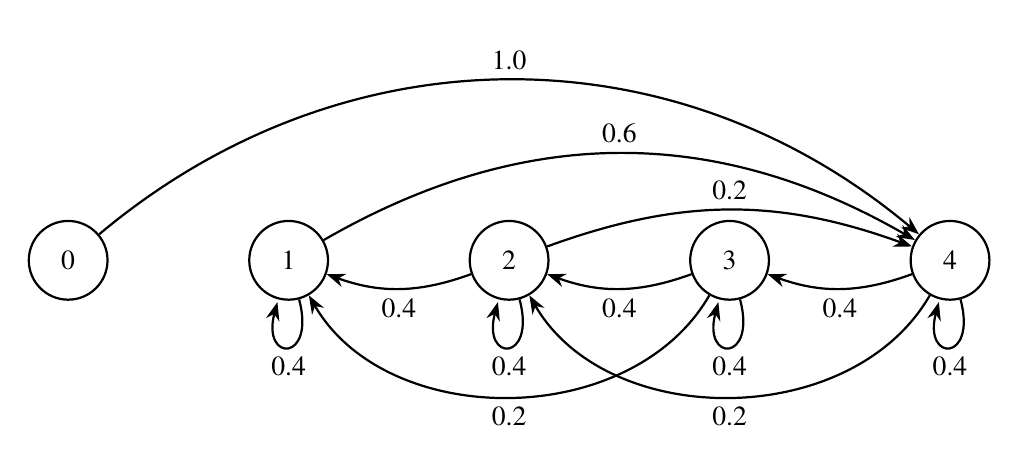
\begin{tikzpicture}[
    ->, 
    >=Stealth, 
    node distance=2.8cm, 
    every state/.style={circle, draw, minimum size=1cm},
    thick
]

% Nodes
\node[circle, draw, minimum size=1cm] (S0) {0};
\node[circle, draw, minimum size=1cm, right of=S0] (S1) {1};
\node[circle, draw, minimum size=1cm, right of=S1] (S2) {2};
\node[circle, draw, minimum size=1cm, right of=S2] (S3) {3};
\node[circle, draw, minimum size=1cm, right of=S3] (S4) {4};

% Transitions from S0
\draw (S0) edge[bend left=40] node[above] {1.0} (S4);

% Transitions from S1
\draw (S1) edge[loop below] node {0.4} (S1);
\draw (S1) edge[bend left=30] node[above] {0.6} (S4);

% Transitions from S2
\draw (S2) edge[bend left=20] node[below] {0.4} (S1);
\draw (S2) edge[loop below] node {0.4} (S2);
\draw (S2) edge[bend left=20] node[above] {0.2} (S4);

% Transitions from S3
\draw (S3) edge[bend left=60] node[below] {0.2} (S1);
\draw (S3) edge[bend left=20] node[below] {0.4} (S2);
\draw (S3) edge[loop below] node {0.4} (S3);

% Transitions from S4
\draw (S4) edge[bend left=60] node[below] {0.2} (S2);
\draw (S4) edge[bend left=20] node[below] {0.4} (S3);
\draw (S4) edge[loop below] node {0.4} (S4);

\end{tikzpicture}
\end{center}
%

\item Find the limiting distribution for the number of rackets in stock when the shop opens, using your transition matrix in (a). 
			\hfill [5 marks]
%
\\
\textbf{Answer:}
\\
To find the limiting distribution, we need to solve the equation:

\begin{align*}
\pi P &= \pi \\
\end{align*}

Where $\pi$ is the limiting distribution vector.

With the constraint that the sum of the probabilities in $\pi$ equals 1:
\begin{align*}
\sum_{i=0}^{4} \pi_i &= 1 \\
\end{align*}


The limiting distribution vector $\pi$ is given by:
\begin{align*}
\pi &= \begin{bmatrix}
\pi_0 & \pi_1 & \pi_2 & \pi_3 & \pi_4 \\
\end{bmatrix}
\end{align*}

We solve the following system of equation using Python numpy:
\begin{align*}
	\pi(P - I) &= 0 \\
	\sum_{i=0}^{4} \pi_i &= 1 \\
\end{align*}

Wolfram Alpha was used to solve the system of equations, using the following code:

\begin{verbatim}
	solve {
p1=0.4p1+0.4p2+0.2p3,
p2=0.4p2+0.4p3+0.2p4,
p3=0.4p3+0.4p4,
p4=0.6p1+0.2p2+0.4p4,
p1+p2+p3+p4=1
} for p1,p2,p3,p4
\end{verbatim}

The solution gives us the limiting distribution: 
\begin{align*}
\pi &= 
\begin{bmatrix}
0 & \frac{10}{43} & \frac{21}{86} & \frac{9}{43} & \frac{27}{86} \\
\end{bmatrix}
\end{align*}

\item Determine the expected long-run average number of restocking orders placed per day. 
			\\\phantom{1}\hfill [2 marks]
%
\\
\textbf{Answer:}
\\
The shop can only restock in a day when it starts with 1 or 2 rackets in stock. The probability of restocking when the day starts with 1 racker in stock is 0.6, and the probability of restocking when the day start with 2 rackets in stock is 0.2. Therefore, the expected long-run average number of restocking order placed per day is given by:

\begin{align*}
E[\text{restocking orders}] &= \pi_1 \cdot 0.6 + \pi_2 \cdot 0.2 \\
&= \frac{10}{43} \cdot 0.6 + \frac{21}{86} \cdot 0.2 \\
&\approx 0.1884 \\
\end{align*}
%

\item If a customer arrives and no rackets are in stock, the sale is lost. Calculate the expected number of lost sales per day in the long run. 
			\hfill [2 marks]
%
\\
\textbf{Answer:}
\\
The only way that a sale can be lost is if the day starts with 1 racket in stock, and someone wants to buy 2 rackets (0.2 probability). Therefore, the expected number of lost sales per day is given by:

\begin{align*}
E[\text{lost sales}] &= \pi_1 \cdot 0.2 \\
&= \frac{10}{43} \cdot 0.2 \\
&\approx 0.04651 \\
\end{align*}

\item Each successful sale generates a profit of $P$, and the delivery charge remains as $C$ regardless of the quantity ordered. Use {\sf Python} to simulate the sales and inventory of this store. Implement two restocking strategies: (i) restock when there are no rackets left, and (ii) restock if there are fewer than two rackets at the end of the day. 
Start with an initial stock of four rackets. Set $P=10$ and $C=15$. Simulate $1000$ days and report the average number of restocking orders, the average number of sales lost, and the average profit from sales. Compare the two restocking strategies based on the simulation results.   
			\hfill [15 marks]
%
\\
\textbf{Answer:}
\\

The following Python code simulates the sales and inventory of the store for both restocking strategies:
\begin{verbatim}
	import numpy as np

# Simulation settings
P = 10
C = 15
N_DAYS = 1000
INITIAL_STOCK = 4

# Demand distribution
demand_values = [0, 1, 2]
demand_probs = [0.4, 0.4, 0.2]

# Simulation function
def simulate(strategy):
    stock = INITIAL_STOCK
    restocks = 0
    lost_sales = 0
    total_sales = 0

    for _ in range(N_DAYS):
        demand = np.random.choice(demand_values, p=demand_probs)
        actual_sales = min(stock, demand)
        lost_sales += demand - actual_sales
        total_sales += actual_sales
        stock -= actual_sales

        # Strategy i - restock if stock == 0
        if strategy == 'strategy_1' and stock == 0:
            stock = 4
            restocks += 1

        # Strategy ii - restock if stock < 2
        elif strategy == 'strategy_2' and stock < 2:
            stock = 4
            restocks += 1

    revenue = total_sales * P
    restock_cost = restocks * C
    profit = revenue - restock_cost

    return {
        'avg_restocks': restocks / N_DAYS,
        'avg_lost_sales': lost_sales / N_DAYS,
        'avg_profit': profit / N_DAYS
    }

# --- MAIN EXECUTION ---
results_strategy_1 = simulate('strategy_1')
results_strategy_2 = simulate('strategy_2')

results_strategy_1, results_strategy_2
\end{verbatim}

The simulation resutls for the two strategies are as follows:

\subsubsection*{Strategy (i): Restock when there are no rackets left}
\begin{verbatim}
{'avg_restocks': 0.192,
  'avg_lost_sales': np.float64(0.041),
  'avg_profit': np.float64(4.83)}
\end{verbatim}

\subsubsection*{Strategy (ii): Restock if there are fewer than two rackets at the end of the day}
\begin{verbatim}
{'avg_restocks': 0.243,
  'avg_lost_sales': np.float64(0.0),
  'avg_profit': np.float64(4.345)}
\end{verbatim}

There is more lost sales with strategy (i) than with strategy (ii), but the average profit is higher with strategy (i) than with strategy (ii). This is because the average number of restocking orders is lower with strategy (i) than with strategy (ii).

\item {\bf (*STAT7003)} To determine the most profitable strategy, derive a condition (expressed in terms of $C$ and $P$) under which the manager should switch from strategy (i) to strategy (ii).   
			\\\phantom{1}\hfill [5 marks] 
%
\\
\textbf{Answer:}
\\

Under strategy (ii), the transition matrix is given by:
\begin{align*}
P_{ii} &= \begin{bmatrix}
0 & 0 & 0 & 0 & 1 \\
0 & 0 & 0 & 0 & 1 \\
0 & 0 & 0.4 & 0 & 0.6 \\
0 & 0 & 0.4 & 0.4 & 0.2 \\
0 & 0 & 0.2 & 0.4 & 0.4 \\
\end{bmatrix}
\end{align*}

The limiting distribution vector $\pi_{ii}$ is given by:
\begin{align*}
\pi^{(ii)} = 
\begin{bmatrix}
0 & 0 & \frac{7}{22} & \frac{3}{11} & \frac{9}{22}
\end{bmatrix}
\end{align*}

Under strategy (ii), the shop can only restock after a day when it starts with 3 rackets in stock, and sells 2 rackets (0.2 probability), or when it starts with 2 rackets in stock and sells 1 or 2 rackets (0.4 and 0.2 probabilities respectively). Therefore, the expected number of restocking orders per day is given by:
\begin{align*}
E[\text{restocks}_{ii}] &= \pi^{(ii)}_2 \cdot 0.6 + \pi^{(ii)}_3 \cdot 0.2 \\
&= \frac{7}{22} \cdot 0.6 + \frac{3}{11} \cdot 0.2 \\
&\approx 0.2455 \\
\end{align*}

We know that since the shop can never start the day with anything less than 2 rackets, the expected number of lost sales for strategy (ii) is 0:
\begin{align*}
E[\text{lost sales}_{ii}] &= 0 \\
\end{align*}

We know that expected demand is given by:
\begin{align*}
E[\text{demand}] &= \sum_{i=0}^{2} i \cdot P(\text{demand} = i) \\
&= 0 \cdot 0.4 + 1 \cdot 0.4 + 2 \cdot 0.2 \\
&= 0.8 \\
\end{align*}

The expected profit from strategy (i) is given by:
\begin{align*}
E[\text{profit}_i] &= P \cdot (E[\text{demand}] - E[\text{lost sales}_i]) - C \cdot E[\text{restocks}_i] \\
\end{align*}

and the expected profit from strategy (ii) is given by:
\begin{align*}
E[\text{profit}_i] &= P \cdot (E[\text{demand}] - E[\text{lost sales}_{ii}]) - C \cdot E[\text{restocks}_ii] \\
&= P \cdot E[\text{demand}] - C \cdot E[\text{restocks}_ii]
\end{align*}

Therefore, the condition under which the manager should switch from strategy (i) to strategy (ii) is given by:

\begin{align*}
E[\text{profit}_i] &< E[\text{profit}_{ii}] \\
P \cdot (- E[\text{lost sales}_i]) &< C \cdot (E[\text{restocks}_i] - \cdot E[\text{restocks}_{ii}]) \\
\frac{P}{C} &< \frac{E[\text{restocks}_i] - \cdot E[\text{restocks}_{ii}]}{- E[\text{lost sales}_i]} \\
&= \frac{0.1884 - 0.2455}{0 - 0.041} \\
& \approx 1.3927
\end{align*}

Therefore, the manager should switch from strategy (i) to strategy (ii) if the ratio $\frac{P}{C} < 1.3927$.

\end{enumerate}

%%%%%%%%%%%%%%%%%%%%
\vspace{5pt}
\newpage
% Q5
%%%%%%%%%%%%%%%%%%%%
\item A smart irrigation system manages water delivery using the following components:
\begin{itemize}
\item two soil moisture sensors (Sensor A and Sensor B) monitors moisture levels. 
\item a central decision unit processes sensor data and determines when irrigation is needed. 
\item two electronic irrigation valves (Valve A and Valve B) which open if instructed. 
\item a power controller provides energy to all components.
\end{itemize}
The system is considered operational if both the power controller and the central decision unit are working, \textbf{and} at least one sensor is working, \textbf{and} at least one valve is working. 
%
\begin{enumerate}
\item Draw a block diagram that represents the system's components and their relationships. 
			\\\phantom{1}\hfill [4 marks] 
%
\\
\textbf{Answer:}
\\

\begin{center}
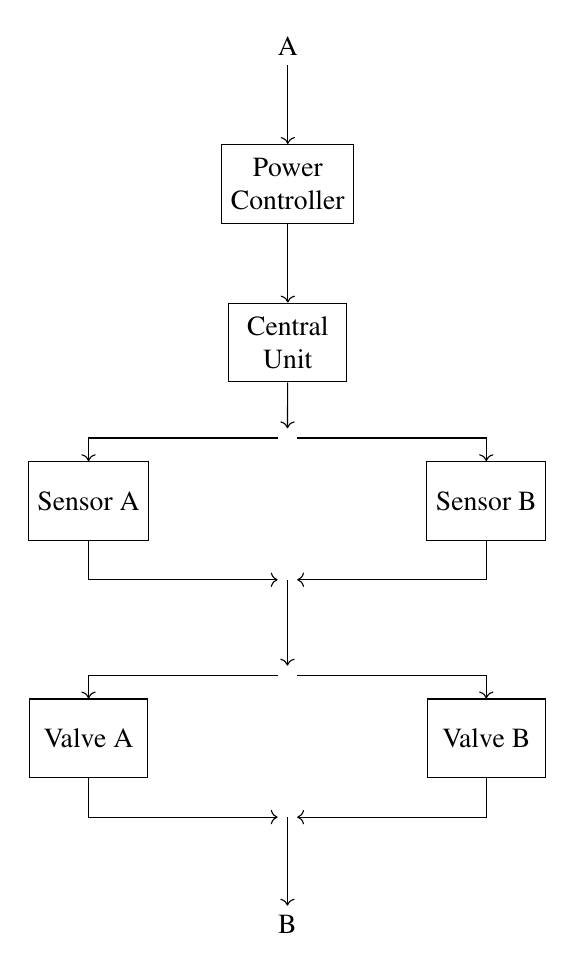
\begin{tikzpicture}[
  component/.style={rectangle, draw, minimum width=1.5cm, minimum height=1cm, align=center},
  conn/.style={draw, thick},
  node distance=1cm
]

% Nodes
\node (A) at (0,0) {A};

\node[component, below=of A] (P) {Power \\ Controller};
\node[component, below=of P] (C) {Central \\ Unit};

% Sensors in parallel
\node[component, below left=1cm and 1cm of C] (S1) {Sensor A};
\node[component, below right=1cm and 1cm of C] (S2) {Sensor B};
\node (Sjoin) at ($(S1)!0.5!(S2)$) {};
\node (Sprejoin) at ($(Sjoin) + (0,+0.8)$) {};
\node (Srejoin) at ($(Sjoin) + (0,-1)$) {};

% Valves in parallel
\node[component, below=2cm of S1] (V1) {Valve A};
\node[component, below=2cm of S2] (V2) {Valve B};
\node (Vjoin) at ($(V1)!0.5!(V2)$) {};
\node (Vprejoin) at ($(Vjoin) + (0,+0.8)$) {};
\node (Vrejoin) at ($(Vjoin) + (0,-1)$) {};

\node (B) [below=2cm of Vjoin] {B};

% Connections
\draw[->] (A) -- (P);
\draw[->] (P) -- (C);
\draw[->] (C) -- (Sprejoin);

% \draw[->] (Sjoin) -- (Vjoin);
\draw[->] (Vrejoin) -| (B);

% Sensor and valve branches
\draw[->] (Sprejoin) -| (S1);
\draw[->] (Sprejoin) -| (S2);

\draw[->] (S1) |- (Srejoin);
\draw[->] (S2) |- (Srejoin);

\draw[->] (Srejoin) -| (Vprejoin);
\draw[->] (Vprejoin) -| (V1);
\draw[->] (Vprejoin) -| (V2);

\draw[->] (V1) |- (Vrejoin);
\draw[->] (V2) |- (Vrejoin);

\end{tikzpicture}
\end{center}

\item Give the structure function for this system.
			\hfill [2 marks] 
%
\\
\textbf{Answer:}
\\
The structure function for the system can be expressed as follows:
\begin{align*}
R_{system} = (1 - (1 - x_{s1})(1 - x_{s2})) \cdot (1 - (1 - x_{v1})(1 - x_{v2})) \cdot (x_{p} \cdot x_{c})
\end{align*}

Where $x_{s1}$ and $x_{s2}$ are the states of Sensor A and Sensor B, respectively, $x_{v1}$ and $x_{v2}$ are the states of Valve A and Valve B, respectively, $x_{p}$ is the state of the Power Controller, and $x_{c}$ is the state of the Central Decision Unit.

\item Assume all six components fail independently and have exponentially distributed lifetimes with mean $\lambda$ years. What is the probability that the system is working at some time $t>0$? 
			\\\phantom{1}\hfill [4 marks] 
%
\\
\textbf{Answer:}
\\
The probability that the system is working at some time $t > 0$ is given by the expression:

\begin{align*}
\Pm(\text{system working at time } t) &= R_{system}(t) \\
\end{align*}

Since the components fail independently and have exponentially distributed lifetimes with mean $\lambda$ years, the reliability function for each component is given by:

\begin{align*}
R_{component}(t) &= e^{-\frac{t}{\lambda}} \\
\end{align*}

The reliability function for the system can be expressed as:
\begin{align*}
R_{system}(t) &= (1 - (1 - R_{s1}(t))(1 - R_{s2}(t))) \cdot (1 - (1 - R_{v1}(t))(1 - R_{v2}(t))) \cdot (R_{p}(t) \cdot R_{c}(t)) \\
&= (1 - (1 - e^{-\frac{t}{\lambda}})(1 - e^{-\frac{t}{\lambda}})) \cdot (1 - (1 - e^{-\frac{t}{\lambda}})(1 - e^{-\frac{t}{\lambda}})) \cdot (e^{-\frac{t}{\lambda}} \cdot e^{-\frac{t}{\lambda}}) \\
&=  e^{-2t/\lambda} \left(2e^{-t/\lambda} - e^{-2t/\lambda}\right)^2
\end{align*}

Therefore, the probability that the system is working at some time $t > 0$ is given by:
\begin{align*}
\Pm(\text{system working at time } t) &= e^{-2t/\lambda} \left(2e^{-t/\lambda} - e^{-2t/\lambda}\right)^2 \\
\end{align*}

\end{enumerate}

%%%%%%%%%%%%%%%%%%%%%%%%%%%%%%%%%%%%%%%%%%%%
%%%%%%%%%%%%%%%%%%%%%%%%%%%%%%%%%%%%%%%%%%%%
%%%%%%%%%%%%%%%%%%%%%%%%%%%%%%%%%%%%%%%%%%%%
\end{enumerate}
\end{document}
